128. \begin{figure}[ht!]
\center{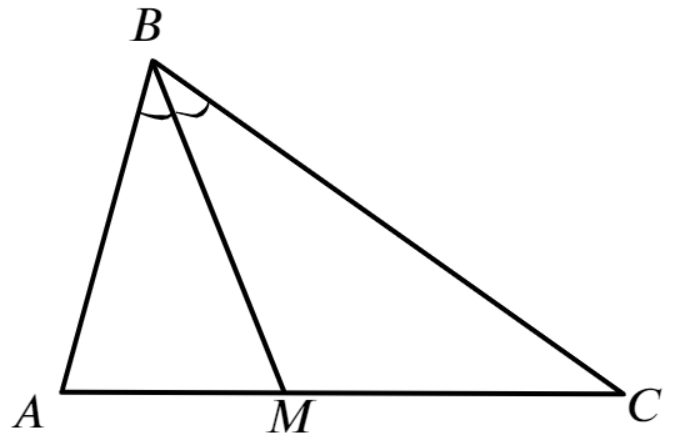
\includegraphics[scale=0.35]{g8-128.png}}
\end{figure}\\
По теореме об основании биссектрисы $\cfrac{AM}{MC}=\cfrac{AB}{AC}.$ У треугольников $ABM$ и $BCM$ общая высота, опущенная из точки $B,$ значит $\cfrac{S_{\Delta ABM}}{S_{\Delta BCM}}=\cfrac{1}{3}=\cfrac{AM}{MC}=\cfrac{AB}{AC},$ значит $AB=AC\cdot \cfrac{1}{3}=12\cdot\cfrac{1}{3}=4\text{ см}.$\\
